\documentclass[11pt,a4paper]{article}
\usepackage[T1]{fontenc}
\usepackage[utf8]{inputenc}
\usepackage{lmodern,microtype}
\usepackage[margin=25mm]{geometry}
\usepackage{graphicx,booktabs,longtable,tabularx,array,amsmath,amssymb}
\usepackage[round,authoryear]{natbib}
\usepackage{xcolor,xurl}
\usepackage[colorlinks=true,linkcolor=black,citecolor=black,urlcolor=blue!45!black]{hyperref}
\usepackage{fancyhdr,caption,enumitem}
\setlength{\parindent}{0pt}
\setlength{\parskip}{5.5pt}
\setlength{\emergencystretch}{2em}
\setlength{\headheight}{14pt}
\pagestyle{fancy}\fancyhf{}
\fancyhead[L]{\small Gupta | Borrowed Standards, Delegated Review}
\fancyhead[R]{\small Research manuscript}
\fancyfoot[C]{\thepage}
\captionsetup{font=small,labelfont=bf}
\setlist{nosep,leftmargin=*}
\newcommand{\USD}{US\$}
\title{\vspace{-1.4em}\textbf{Borrowed Standards, Delegated Review}\\[.45em]
\large Complaint Routing and Evidentiary Participation in\\Central Asia's Infrastructure Transition}
\author{Shivam Gupta\\\small Independent Researcher, India\\\small\href{mailto:shivam1720406@gmail.com}{shivam1720406@gmail.com}}
\date{16 October 2026}
\begin{document}
\maketitle
\begin{abstract}
\noindent Infrastructure can adopt a financier's safeguards without assigning complaints to that financier's accountability mechanism. This paper examines that distinction through a reproducible reconstruction of AIIB's end-2024 and end-2025 cofinancing registers and a documentary process trace of Kazakhstan's Shokpar wind project. Of 26 Central Asian and Mongolian entries in the later register, 23 designate another institution's mechanism, representing \USD4,740.28 million of \USD5,417.78 million in listed AIIB financing. These are forum designations, not findings of harm or missing remedy. Across the global register, no deterministic lookup using only the published applicable-policy label can reproduce all forum designations: at least 14 of 152 entries must be misclassified. Matching all 136 earlier entries finds no change in their policy or forum labels; the regional shift reflects added operations. Shokpar demonstrates why successful routing is insufficient as an accountability endpoint. Its complaint was forwarded from AIIB to EBRD's IPAM, but the closure report later records unequal access to monitoring reports, discontinued problem solving, and transfer toward compliance assessment. Reading these records against the 2026 PPM rules distinguishes coordination from findings-triggered institutional learning. The contribution is an auditable regional dataset, a bounded measurement result, and a practical reporting framework separating applicable norms, review mandate, evidence access, and remedial outcome.
\end{abstract}
\noindent\textbf{Keywords:} infrastructure finance; Central Asia; AIIB; independent accountability mechanisms; wind energy; evidence access; just transition

\section{Introduction}
An infrastructure project can display several financiers' names while presenting affected people with a single designated institutional route for environmental and social complaints. Conversely, it can adopt another bank's safeguards while retaining review through the Asian Infrastructure Investment Bank's Project-affected People's Mechanism (AIIB PPM). The financial partnership, the applicable standard, and the forum for reviewing institutional conduct are related arrangements, but they are not interchangeable descriptions of the same thing. Their differences matter when people need to challenge how a transition project has been assessed or managed.

This paper investigates how those arrangements are made visible in Central Asia and Mongolia, and what remains unresolved after a complaint reaches the designated forum. It combines two scales of evidence. A reconstruction of AIIB's published cofinancing registers establishes the distribution and limits of recorded forum designations. A process trace of Shokpar, a 100 MW wind project in southern Kazakhstan, follows an actual complaint from receipt by AIIB to EBRD's Independent Project Accountability Mechanism (IPAM), and then to a dispute over the evidence available to the parties. The combination links the architecture of finance to the practical conditions of participation without treating a registry field as a measure of lived access.

The distinction is especially relevant to infrastructure promoted as green. The issue in Shokpar is not whether wind generation can displace fossil electricity. It is whether the actors contesting a project's biodiversity assessments can inspect the information through which their concerns are evaluated. International finance can bring assessment requirements and an external forum into a project. Those institutional additions do not by themselves settle who controls the production, circulation, or interpretation of subsequent monitoring evidence.

The research questions are: \emph{RQ1}, how do AIIB's published policy and forum designations relate in the regional register, and can one be recovered from the other? \emph{RQ2}, does a changing aggregate picture reflect revised designations for existing entries or a changing composition of operations? \emph{RQ3}, what does Shokpar reveal about the relationship between successful referral, access to evidence, and progression toward remedy?

The findings are specific. Twenty-three of 26 regional entries in the end-2025 register designate a mechanism other than PPM. That is neither evidence that 23 projects lack an accountability route nor an estimate of the performance of those routes. Within the global register, the same published policy label can accompany different designated mechanisms. Matching the earlier register shows that a substantial change in the regional financing-weighted share occurs without any changed designation among matched entries. Finally, Shokpar provides evidence of a working referral followed by a consequential participation problem within the receiving process. A simple opposition between access and exclusion cannot describe this sequence adequately.

The paper contributes a new, source-linked regional reconstruction and a joined analysis of register designations, a documented complaint trajectory, and the revised 2026 PPM rules. It does not claim to discover cofinancing exclusions, the general importance of evidence, or the distinction between access and remedy. Its methodological contribution is to make those distinctions operational and falsifiable in a concrete infrastructure-finance setting. The resulting Accountability Route Ledger is an open implementation for retaining the source and scope of a designation rather than generating legal conclusions from lender identity.

\section{Literature and analytical position}
\subsection{Institutional convergence is not a sufficient account of accountability}
Scholarship has already moved beyond a simple question of whether AIIB copies or challenges established development banks. \citet{ransdell2019} examines institutional innovations and their implications for cooperation. \citet{gu2023} interprets AIIB's environmental and social framework as a combination of inherited arrangements and institutional innovation. \citet{creutz2023}, examining rights protection, emphasizes fragmentation and the tension between efficiency and protection. These accounts direct attention to the institutional meaning of an adopted safeguard rather than its presence alone.

Recent comparative work further establishes that convergence in the language and structure of environmental and social frameworks can coexist with a distinctive position in development finance \citep{lee2025}. The question here is narrower than whether institutional convergence has occurred. It is whether the \emph{published applicable-policy label} is sufficient to identify the forum AIIB designates for complaints under a particular operation. An empirical failure of that mapping does not disprove normative convergence. It identifies an additional institutional relationship that convergence measures need to preserve.

\subsection{Cofinancing exclusions and remedial limits are established problems}
The closest prior work is not confined to academic journals. \citet{geary2023} analyze AIIB's portfolio, the cofinancing exclusion, project-level barriers, and confusing distinctions among cofinanciers and instruments. Their report explicitly identifies that adoption of a partner's safeguards does not settle whether PPM is available. It also discusses difficulties that can persist when a complaint is directed elsewhere. Consequently, neither the existence of the exclusion nor a generic claim that cofinancing creates complexity is a defensible novelty claim for this paper.

Earlier legal scholarship connects the promise of Southern development institutions to their capacity to give affected communities meaningful channels of redress \citep{mirza2018}. \citet{lorenzo2024} distinguishes institutional answerability from liability and identifies limits in the remedial role of accountability mechanisms. OHCHR's guidance likewise treats remedy as an institutional ecosystem extending beyond the availability of a complaint channel \citep{ohchr2022}. These works support separating an institution's capacity to receive or investigate a complaint from the measures eventually available to address harm.

The incremental contribution here is a later regional census of published designations, checked against an earlier snapshot, and a process trace extending through Shokpar's 2026 problem-solving closure. This trace permits examination of a specific downstream issue: the circulation of monitoring reports among the client, mechanism, management, and requesters. It also allows a careful comparison with the new distinction between ordinary coordination and the management-report trigger following a cofinancier's noncompliance finding. These are developments beyond the 2023 portfolio analysis, rather than a replacement for it.

\subsection{A regional account of procedural power}
Central Asian climate and energy politics cannot be reduced to a competition between national origins of capital. \citet{skalamera2025} links international climate relationships to domestic distributional tensions in Kazakhstan and Uzbekistan. Regional work on just transition also emphasizes that institutional terminology may travel differently from the everyday concerns through which civil society understands fairness \citep{ponedelnik2026}. The present paper takes procedural power as a concrete object: the institutional capacity to make a contested project assessment answerable and the evidentiary conditions under which that contest proceeds.

The case involves a Chinese state-owned corporate sponsor, a multilateral institution initiated by China, an established European development bank, Kazakh institutions, and a local conservation organization. These are distinct roles. Sponsor nationality does not determine the applicable safeguards or the complaint forum. Nor should AIIB be equated with Chinese policy-bank lending, or either with Russian or Eurasian finance. This study observes arrangements inside one multilateral cofinancing architecture. It does not rank national financing models or generalize to bilateral lending whose contracts have not been examined.

This specificity also limits the social claims. Shokpar's public complaint concerns biodiversity assessment and project categorization. The reviewed record does not establish impacts on herders' tenure, gendered displacement, or workers' conditions. Those questions remain important, but inserting them into this case without evidence would obscure rather than strengthen its contribution to the workshop's concern with whose knowledge and claims count.

\section{Sources and research design}
\subsection{A census of two registers, not the entire AIIB portfolio}
The primary quantitative source is AIIB's \emph{Co-Financed Projects (End-2025)} register, whose download filename bears 11 March 2026. It contains 152 numbered entries, with fields for member, project, sector, financing type, lead cofinancier, AIIB financing, approval date, environmental and social reference institution, applicable policy, and applicable independent accountability mechanism (IAM). The historical comparator is its updated end-2024 register of 136 entries \citep{register2025,register2024}. Both were retrieved on 16 October 2026. The observation period named by a register is distinguished from its publication or retrieval date.

The regional subset includes Kazakhstan, the Kyrgyz Republic, Tajikistan, Turkmenistan, Uzbekistan, and Mongolia. The geographical definition covers the five Central Asian republics plus Mongolia; it excludes Azerbaijan and other corridor-connected states. The extraction includes every numbered entry satisfying that country definition, irrespective of sector or financing instrument. This avoids selecting only operations presented as renewable infrastructure after observing their complaint route.

The denominator is deliberately restricted. These documents organize entries by partner lead institution. They are not a census of all AIIB lending, all cofinancing in the region, or all infrastructure. The omission of a project cannot establish that it has no cofinanciers. Zhanatas, for example, is absent from these registers even though AIIB's own account describes a financing partnership involving EBRD and the Eurasian Development Bank \citep{aiib2019impact}. No claim about that project's mechanism is derived from its absence. Likewise, the absence of a Turkmenistan entry and the presence of only crisis-response operations for Mongolia describe the source, not either country's complete infrastructure-finance landscape.

The unit is a numbered financing entry, not necessarily a unique physical installation. Additional facilities can appear separately elsewhere in the global register; one portfolio entry can cover several plants. Amounts are the register's listed AIIB financing in USD millions. They are not total project costs, current outstanding exposure, disbursements, remedial budgets, or amounts associated with demonstrated harm.

\subsection{Extraction, verification, and snapshot linkage}
The pipeline uses PyMuPDF's table geometry to extract and flatten cell text while retaining source page, row number, and file SHA-256. A second text engine, Poppler's \texttt{pdftotext}, independently checks each numbered line's amount, approval date, reference institution, applicable-policy label, and IAM. Those checks pass for all 288 row observations across the two snapshots. They test extraction agreement, not the bank's substantive legal determinations.

The 26 later regional entries were additionally checked against rendered register pages, with their member, financing, policy, and IAM recorded in a separate fixture. This is a second verification pass within the same study, not independent intercoder validation. No inter-rater reliability statistic is claimed. Labels are preserved as published; full policy versions are not inferred from abbreviated labels such as ``EBRD ESP.''

For linkage, the key is the exact tuple of member, project title, approval date, and listed amount. All 136 earlier entries match uniquely to the later register. Using member, date, and amount alone would create collisions: the Sirdarya power and medium-size cities entries, for example, share those three fields. Retaining the title avoids falsely joining distinct operations. A changed title or amount would require explicit adjudication; no such repair is needed for the matched set here.

The analysis is exploratory documentary research. The country definition and alternative denominators are explicit, but this is not a preregistered evaluation or a probability sample. The numerical results are exact descriptions of the extracted registers. Confidence intervals and significance tests would not address the main uncertainties, which concern source coverage, classification, and the distance between published designations and practical access.

\subsection{Process tracing and source hierarchy}
The Shokpar trace draws on AIIB's project description, IPAM's case registry, its 2025 assessment report, and its problem-solving closure report dated April 2026 and listed in the registry on 22 June 2026 \citep{shokparproject,shokparregistry,shokparassessment,shokparclosure}. The evidence ledger preserves document identifiers and printed-page locators. Exact dates are used only when the record gives them. Month-level observations remain intervals; a first day is never treated as an observed event date merely to draw a timeline.

The reports are authoritative evidence of the mechanism's recorded handling and its account of the parties' positions. They are not an independent ecological assessment. Allegations, client responses, bank-management explanations, administrative events, and findings are therefore coded separately. The four underlying monitoring reports described in the closure document were not obtained for this study. No conclusion about their scientific quality, the actual mortality rate, or the adequacy of a specific mitigation technology follows from their recorded circulation.

For interpretation of current institutional design, the study reads the PPM policy and rules effective 1 January 2026 alongside the 2018 policy \citep{ppm2026,rules2026,ppm2018}. The revised documents expressly apply to submissions made on or after 1 January 2026. Shokpar's initial submission predates that date. Its historical handling is not retroactively assessed as a breach of the revised rules; the later rules are used to examine the architecture facing new submissions and to identify reporting questions raised by the case.

\section{Separating the objects of accountability}
Figure~\ref{fig:layers} distinguishes four questions. \emph{Applicable norms} identify the requirements used to assess and manage risks. \emph{Review mandate} identifies the institution and conduct subject to a mechanism's review. \emph{Evidentiary participation} concerns who can inspect and contest relevant information. \emph{Outcome} concerns an agreement, finding, implementation measure, or remedy. A complaint can move between processes, and a negotiated outcome need not follow a compliance finding. The figure is an analytical sequence of questions, not a mandatory sequence of institutional stages.

\begin{figure}[htbp]\centering
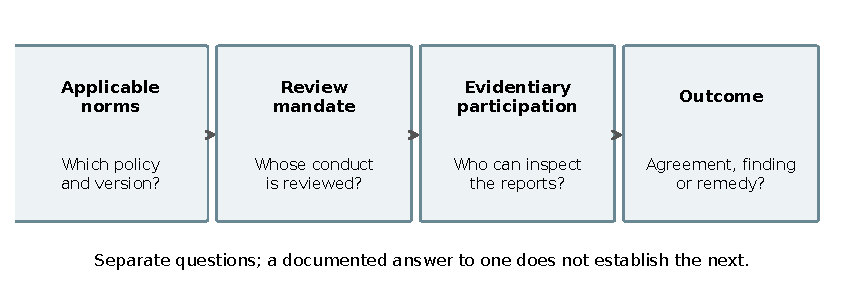
\includegraphics[width=\linewidth]{../figures/accountability_layers.pdf}
\caption{Four distinct objects of accountability. A policy label does not establish a forum; a forum designation does not establish equal access to evidence or a remedial outcome. Source: author's analytical framework.}\label{fig:layers}
\end{figure}

For a register entry $i$, let $s_i$ denote its published applicable-policy label, $m_i$ its AIIB-designated IAM, and $a_i$ its listed financing. The mapping $s_i\mapsto m_i$ is an empirical question. A designation is not a decision on an actual requester's eligibility. The latter can depend on standing, dates, prior engagement, subject matter, and the mechanism's mandate. Nor does the single IAM column enumerate all possible routes under another financier's own policies, domestic law, or other remedial arrangements.

A simple diagnostic quantifies the information lost by replacing the IAM field with a deterministic lookup on policy label alone. Define $n_{sm}=|\{i:s_i=s,m_i=m\}|$. The smallest possible number of disagreements with the register is
\begin{equation}
E_s=\min_f\sum_i\mathbf{1}\{f(s_i)\ne m_i\}
=\sum_s\left(\sum_m n_{sm}-\max_m n_{sm}\right).
\label{eq:error}
\end{equation}
Each policy group must receive one prediction. Choosing its most frequent IAM minimizes that group's errors independently; summing proves the identity. A weighted version replaces counts with sums of $a_i$. This elementary calculation is not a new learning algorithm. It is a finite-register test of whether a proposed simplification preserves the published information. It says nothing about a classifier that also observes project-specific agreements or sufficiently detailed institutional histories.

The institutional distinction is explicit in the 2026 rules. Section 11.2 addresses agreement both to apply a cofinancier's policies and to rely on its IAM. Section 11.4 separately addresses use of partner policies without an agreement to use the partner IAM: PPM then considers AIIB's due diligence and monitoring against the agreed policies. Thus, policy borrowing and forum delegation are separate institutional operations \citep[secs.~11.1--11.4]{rules2026}. Collapsing them loses information that the rules themselves preserve.

\section{Results: the regional architecture and its measurement}
\subsection{The same published safeguards can lead to different designated forums}
The end-2025 global register lists 30 entries designating AIIB PPM and 122 designating another institution's mechanism. Eleven of 54 entries under ADB's Safeguard Policy Statement designate PPM, as do three of 19 entries under EBRD's policy. All 12 entries using the IFC policy-and-performance-standards label designate PPM. Four further entries use AIIB's own policy and PPM. Figure~\ref{fig:matrix} presents the complete cross-tabulation.

\begin{figure}[htbp]\centering
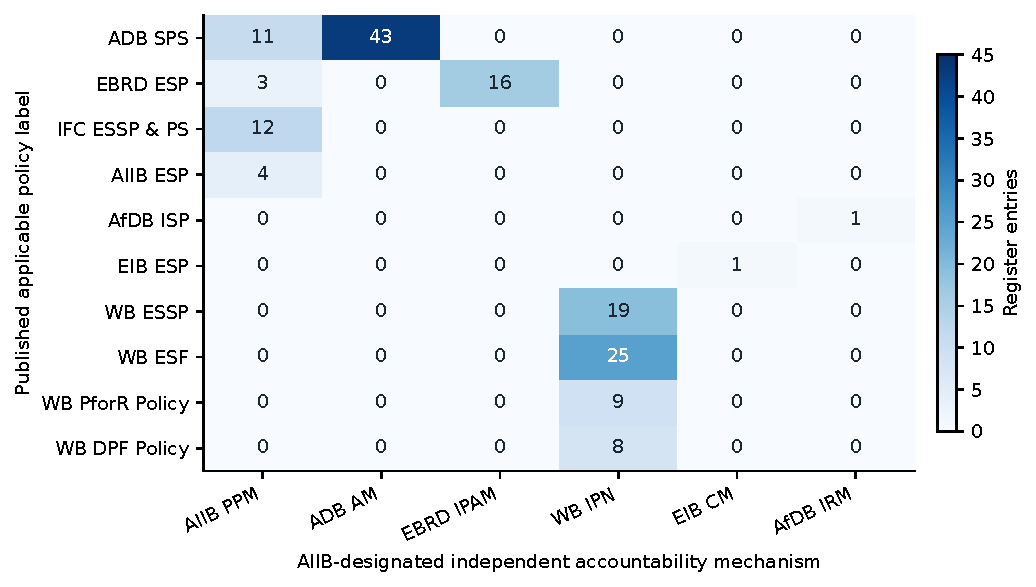
\includegraphics[width=.94\linewidth]{../figures/policy_forum.pdf}
\caption{Published policy labels and AIIB-designated IAMs, end-2025 register ($n=152$). Cells are entry counts, including explicit zeros. These are institutional designations rather than observations of eligible complaints. Source: reconstruction of \citet{register2025}.}\label{fig:matrix}
\end{figure}

Equation~\ref{eq:error} gives $E_s=11+3=14$, or 9.21\% of the register. The minimum financing-weighted disagreement is \USD1,162.70 million. These are the optima over every policy-label-only deterministic lookup, not the measured error of an operational advice service. A more naive rule assigning every policy to its issuing institution's IAM disagrees with 26 entries (17.11\%). Adding the published financing-type field reduces the minimum count to seven, but does not eliminate ambiguity. Neither result establishes that project history could never resolve the distinction. It establishes that these particular fields do not do so by themselves.

There is a regional counterexample within EBRD-policy entries. Dushanbe--Uzbekistan Border Road Improvement designates PPM, while Shokpar designates IPAM. The Dushanbe approval summary expressly adopts EBRD's 2008 policy \citep{dushanbe2016}; Shokpar's documentation refers to the later EBRD framework. Their common abbreviated register label therefore should not be mistaken for identical policy versions. The precise empirical conclusion concerns the insufficiency of the \emph{published label}, not an assertion that otherwise identical legal instruments have conflicting meanings.

\subsection{Regional finance is predominantly designated to partner mechanisms}
The later register contains 26 regional entries and \USD5,417.78 million in listed AIIB financing. Twenty-three entries (88.46\%) designate a partner mechanism; their financing totals \USD4,740.28 million (87.49\%). The three PPM-designated entries are Dushanbe road (\USD27.50 million), Almaty railway bypass (\USD150 million), and Uzbekistan's green and resilient market economy climate policy-based financing (\USD500 million).

\begin{table}[htbp]\centering\small
\caption{Regional entries by member, end-2025 register. Amounts are listed AIIB financing in USD millions. ``Partner IAM'' means the IAM designated by AIIB is not PPM; it does not mean that PPM exclusion removes every remedial route.}\label{tab:country}
\begin{tabular}{lrrrr}\toprule
Member & Entries & Financing & Partner IAM entries & Partner IAM financing\\\midrule
Kazakhstan & 7 & 2,503.90 & 6 & 2,353.90\\
Kyrgyz Republic & 3 & 150.00 & 3 & 150.00\\
Mongolia & 3 & 221.00 & 3 & 221.00\\
Tajikistan & 3 & 357.50 & 2 & 330.00\\
Turkmenistan & 0 & 0.00 & 0 & 0.00\\
Uzbekistan & 10 & 2,185.38 & 9 & 1,685.38\\\midrule
Total & 26 & 5,417.78 & 23 & 4,740.28\\\bottomrule
\end{tabular}
\end{table}

The distribution in Table~\ref{tab:country} and Figure~\ref{fig:regional} reflects several instruments. Mongolia's three entries concern crisis response, vaccines, and exogenous shocks. They do not provide a sample of Mongolian mines, transmission corridors, or renewable plants. The inclusion of such entries is useful for describing the register, but it makes an unqualified ``green infrastructure'' denominator inappropriate.

\begin{figure}[htbp]\centering
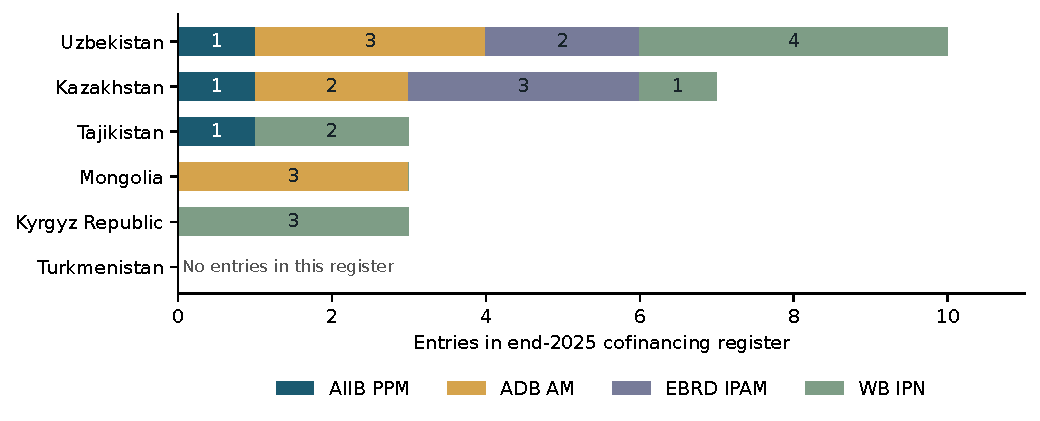
\includegraphics[width=.94\linewidth]{../figures/regional_routes.pdf}
\caption{The distribution of AIIB-designated forums across the defined region. A zero means no entry in this register, not no lending or no remedy. Source: end-2025 register reconstruction.}\label{fig:regional}
\end{figure}

Table~\ref{tab:scopes} therefore reports alternative scopes. Excluding all sectors beginning ``CRF-'' leaves 17 entries, of which 14 designate a partner IAM. Restricting to the published Energy or Transport labels leaves 11 entries, of which eight designate a partner mechanism. But that subset includes Uzbekistan's \USD500 million climate policy operation. Removing it leaves ten entries and raises the financing-weighted partner-designation share from 72.91\% to 91.13\%. This large difference is a denominator effect, not evidence of stronger or weaker accountability in one set of communities.

\begin{table}[htbp]\centering\small
\caption{Sensitivity to the operation boundary. All figures describe the end-2025 regional register. ``Generation'' excludes the policy-based operation and retains the five named generation or rehabilitation entries, including Sirdarya gas.}\label{tab:scopes}
\begin{tabular}{p{6.6cm}rrr}\toprule
Scope & Entries & Partner entries & Partner financing share\\\midrule
All regional entries &26&23&87.49\%\\
Exclude CRF-labeled sectors &17&14&78.47\%\\
Energy or Transport labels &11&8&72.91\%\\
Energy or Transport, excluding climate policy operation &10&8&91.13\%\\
Generation and rehabilitation entries &5&5&100.00\%\\\bottomrule
\end{tabular}
\end{table}

The generation subset totals \USD615 million: Sirdarya gas (100), Masdar solar (145), Shokpar wind (40), Nurek rehabilitation (60), and Rogun development (270). It is not labeled a renewables-only cohort. Project-page checks also show why sector metadata should not be silently harmonized. The register labels Uzbekistan's climate policy operation Energy, whereas its current project page labels it Multi-sector and describes policy and governance reforms \citep{uzbekcpbf}. The raw register classification is retained; the instrument-specific exclusion is reported explicitly.

\subsection{The change between snapshots is compositional}
The earlier regional register contains 21 entries totaling \USD4,217.78 million. Only Dushanbe road designates PPM, leaving 95.24\% of entries and 99.35\% of listed financing designated to partner mechanisms. In the later regional register those shares are 88.46\% and 87.49\%. Reading this movement as a jurisdictional reform would be mistaken.

All 136 earlier entries match to the later global register, with no change in their applicable-policy or IAM labels. In the regional subset, five added operations account for the entire difference: Kazakhstan's M-32 highway and Almaty bypass, the Kyrgyz Republic's water and sanitation and sustainable-finance operations, and Uzbekistan's climate policy financing. The two new regional PPM entries add \USD650 million. Among the matched regional entries, the old pattern remains exactly unchanged. At global scale, one of the sixteen added register entries has a 2024 approval date, which also cautions against interpreting additions to a register as a clean annual flow of new approvals.

This comparison cannot rule out an unreported contractual amendment or a practical change in access. It rules out a much narrower explanation: that the aggregate change is produced by changed \emph{published designations} for the matched entries. The distinction is important when a new institutional policy and a changing portfolio become visible at roughly the same time. Temporal proximity does not identify policy effect.

\section{Shokpar: after a complaint reaches the right institution}
\subsection{An actual referral, with a contested assessment}
Shokpar is a 100 MW wind project developed by China Power International Holding and Visor. AIIB describes the former as a subsidiary of China's State Power Investment Corporation and records adoption of EBRD's environmental and social requirements for the cofinanced project \citep{shokparproject}. IPAM's assessment records different positions on bird risks, project categorization, and mitigation: requesters argued for stronger assessment and protective measures, while the client and EBRD management defended their assessment and categorization \citep[pp.~8--11]{shokparassessment}. These are contested positions, not findings adopted here.

The closure report identifies receipt by AIIB's mechanism on 13 May 2024 and forwarding to IPAM on 29 May. IPAM suspended registration on 17 July to allow management and client engagement, then registered the request on 22 October. The elapsed intervals are 16 days from initial receipt to referral and 162 days from initial receipt to registration; 97 of the latter days follow the recorded suspension. These are calendar intervals, not findings that deadlines were violated or that delegation caused the duration.

The observed referral is analytically important. It prevents an inference that ineligibility for PPM consideration meant the complaint simply vanished. IPAM became an operative forum. EBRD's public explanation of mutual reliance also describes this routing arrangement \citep{ipamcollaboration}. The case therefore permits a more demanding question than whether a complaint channel exists: what conditions governed participation after the handoff?

\begin{figure}[htbp]\centering
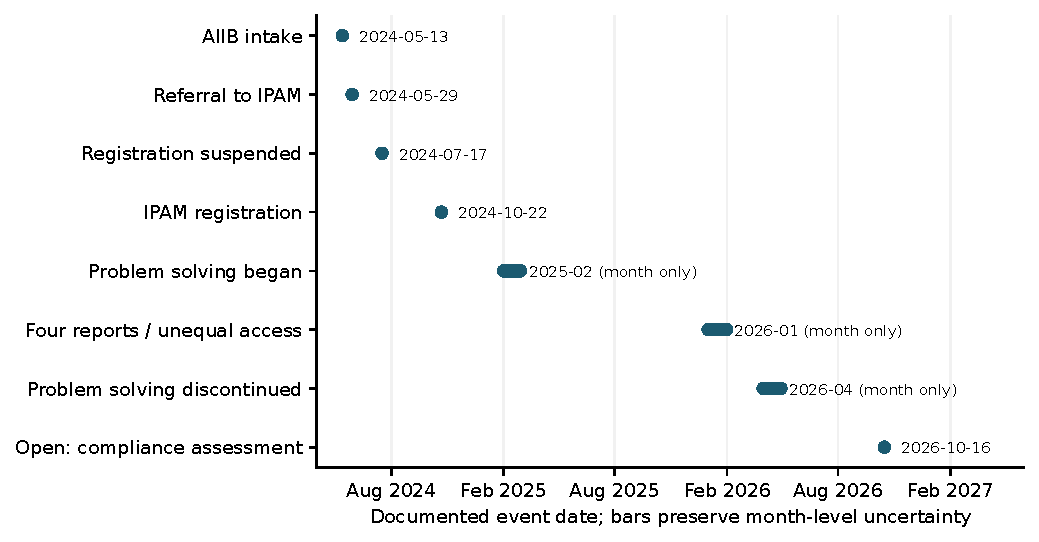
\includegraphics[width=\linewidth]{../figures/shokpar_timeline.pdf}
\caption{Selected documented events in IPAM case 2024/05. Horizontal marks preserve month-only dates; exact dates are individually labeled. The case remained open at compliance assessment in the 16 October 2026 registry snapshot. Sources: IPAM closure report, printed pp.~7--8, and case tracker.}\label{fig:timeline}
\end{figure}

\subsection{Monitoring evidence and the terms of participation}
The 2026 closure document records a sequence in which monitoring studies were undertaken, the client supplied four reports to IPAM and EBRD management in January 2026, and requesters received summaries rather than the full versions. It reports disagreement over the shared findings and persistent difficulties in trust. A February mission involved separate meetings with the parties. In April, requesters discontinued problem solving and sought progression to compliance. The registry subsequently marked problem solving as having reached no agreement and showed the case at compliance assessment \citep[pp.~7--8]{shokparclosure}; \citep{shokparregistry}.

The distinction between reports reaching the mechanism and reports reaching requesters is the central evidentiary observation. A monitoring commitment can produce new information without giving the parties equivalent capacity to evaluate it. A summary may communicate a result while withholding the methods, observations, or qualifications necessary to challenge it. Because the underlying reports were not inspected, this study does not determine which such elements were absent here. It establishes the narrower documented asymmetry in access to full reports.

That asymmetry supplies evidence of a participation bottleneck, but it does not isolate its causal effect. Trust difficulties preceded the final exchange; the client did not describe its commitment to formal problem solving in the same way as the requesters' willingness to engage. The public material does not provide an otherwise equivalent negotiation in which full reports were shared. It therefore cannot establish that disclosure alone would have produced an agreement, that either party acted in bad faith, or that a particular conservation measure was required. The process trace locates an obstacle and an institutional question; it does not estimate a treatment effect.

The case also distinguishes the end of a function from the end of accountability. Problem-solving closure did not close the case. The move toward compliance assessment opened a different question concerning bank adherence to its requirements. As of the retrieval cutoff, the examined record did not supply a final compliance determination or an implemented settlement. Labeling the whole process either a completed remedy or an absence of any review would erase its actual procedural state.

\subsection{Coordination and findings-triggered learning}
The 2026 PPM architecture distinguishes two feedback obligations. Policy section 11.1 provides for coordination with a relied-upon IAM and reporting the outcome of its review to AIIB's Board. Section 11.2 adds a management report on implications for AIIB and institutional learning when the cofinancier's mechanism makes a noncompliance finding. Rules sections 11.3 and 11.5 elaborate the distinction, including an opportunity for PPM to comment on the latter report \citep{ppm2026,rules2026}.

These provisions should not be collapsed into a claim that nothing must be reported until noncompliance is found. The broader coordination and outcome-reporting provision remains. Conversely, the additional management-report trigger cannot be treated as equivalent to evidence access, an agreement, or compensation. For new submissions under the revised rules, its trigger is a specific institutional finding. A prolonged negotiation or a move into compliance assessment does not by itself establish that this trigger has occurred.

Shokpar motivates this distinction but does not establish a breach of either new provision. Its submission was made in 2024; the revised policy's temporal scope is explicit. This paper does not determine the application of the new reporting provision to legacy referrals, and absence of a report in the sources examined would not prove absence of internal coordination. The supported design implication is prospective: reporting should make an intermediate impasse visible without confusing it with a finding, and should identify which institution retains responsibility for the next action.

\section{Discussion: accountability as a continuing relation}
\subsection{From locating a forum to sustaining contestability}
The evidence supports a two-part argument. First, accountability in the cofinancing architecture is relational: the norm used, the institution reviewing conduct, and the bank supplying finance need not coincide. Second, institutional referral does not exhaust procedural participation. The ability to inspect and contest evidence can remain uneven after the correct forum has received a complaint.

The first point qualifies geopolitical shortcuts. In Shokpar, Chinese corporate participation coexists with EBRD standards and an EBRD forum. In Dushanbe road, an EBRD policy label coexists with PPM designation. Almaty's project page describes assessment against AIIB requirements as well as IFC policies, while the register designates AIIB policy and PPM \citep{almaty}. No single label for national origin, institutional leadership, or policy family captures these relationships. This is an argument for examining the operative arrangement, not for assuming that a Western policy label guarantees substantive protection.

The second point concerns just transition as an ability to contest project knowledge. Affected actors are not only recipients of compensation or consultees before approval. They can generate observations, challenge a risk assessment, and question a proposed mitigation hierarchy. Participation in that capacity requires more than an invitation to negotiate. It requires intelligible information and conditions under which contrary evidence can be examined. Shokpar's recorded dispute is therefore relevant to the distribution of authority within green infrastructure, even though the paper does not adjudicate the environmental claims themselves.

These conclusions do not show that multiple full investigations would always be preferable to reliance on one forum. Duplication can increase burdens on complainants and institutions alike. A defensible arrangement could combine a clear entry point with shared institutional leverage and accessible evidence. The empirical issue is whether coordination sustains those conditions, rather than whether institutional multiplicity is intrinsically beneficial.

\subsection{A practical Accountability Route Ledger}
The released implementation treats the source-linked designation as a record with explicit limits. It retains snapshot, project identifier, policy label, mechanism, source locator, and file hash. An absent mechanism or source yields ``unresolved,'' not a denial of eligibility. A lookup can return the recorded forum without predicting an actual complainant's admissibility. Case events retain date precision and distinguish referral, registration, problem-solving closure, and case status.

For institutional use, the schema should extend to policy versions, review target, evidence-production commitments, report recipients, requester access, the present function, findings, follow-up obligations, and documented implementation. The paper's prototype demonstrates the register and event components; it does not claim automatic extraction of undisclosed agreements or legal reasoning over every mechanism. Its small interface makes the important restriction testable: a safeguard label alone cannot generate a forum determination.

Three reporting changes follow directly from the findings. A project disclosure should identify the adopted norm and designated mechanism separately, including the source of any reliance arrangement. Monitoring commitments made during a complaint should specify which parties will receive full reports, any justified confidentiality restrictions, and a procedure to challenge a withheld version. Finally, a public status record should distinguish a function ending without agreement from a finding or completed remedy, and name the institution responsible for the next procedural step. These are proposals for institutional practice, not assertions that every reviewed loan contract already creates those duties.

There are practical applications for affected-community advisers, sustainability consultants, lender supervision teams, and developers preparing disclosure packages. Existing resources such as Accountability Counsel's complaint database and the Early Warning System already provide project and complaint discovery \citep{console,ews}. The proposed ledger complements them by preserving the evidence for policy--forum relations and intermediate procedural states. A commercial implementation could provide version monitoring and quality assurance, but this study does not establish customer demand, procurement willingness, a market size, patentability, or improved remedial outcomes. Access to the underlying evidence should remain inspectable by the people whose complaints are represented.

\section{Limits and conclusions}
The quantitative coverage is one institution's public cofinancing register. Neither the register nor this study establishes the distribution of all Chinese, Russian, Eurasian, Gulf, domestic, or multilateral infrastructure finance. Its abbreviated labels can omit legally significant distinctions. Published designations are not current eligibility determinations, and financing-weighted descriptions are not harm-weighted measures. The policy-operation sensitivity demonstrates how instrument mix can materially change an infrastructure comparison.

The qualitative case is selected because it documents an actual cross-institution referral and a subsequent evidentiary dispute. It is not representative of all referred complaints. Institutional reports mediate the parties' accounts, and the underlying monitoring reports remain outside this study's evidence. A final ecological judgment, an account of local experience beyond the public record, and a causal evaluation of reliance arrangements would require additional evidence. The reproducible audit strengthens the transparency of this limited study; it does not remove those limits.

Within that scope, the results are conclusive about three matters: the published policy label is insufficient to reproduce designated forums; the regional aggregate change between these snapshots occurs without changed labels among matched entries; and Shokpar records successful referral followed by unequal access to full monitoring reports and a transition away from problem solving. Together they show why the reach of sustainability standards cannot be assessed by naming a policy or locating a mechanism alone. Accountability must also be followed through the conditions under which project knowledge is shared, challenged, and connected to subsequent institutional action.

\paragraph{Data and code availability.} The extraction scripts, factual register reconstructions, event ledger, source manifest, figures, tests, and manuscript source are available at \url{https://github.com/shi1720/accountability-route-ledger}. Source documents are identified by URL and SHA-256; third-party documents retain their own rights. Offline analysis runs from the released CSV and JSON files. Extraction from the original PDFs additionally requires PyMuPDF and Poppler.

\paragraph{Author affiliation and interests.} Shivam Gupta is an independent researcher and founder of Siloed. The study does not evaluate a Siloed product or report commercial validation of the proposed ledger.

\bibliographystyle{plainnat}
\bibliography{references}

\appendix
\section{Regional register reconstruction}
Table~\ref{tab:appendix} gives every regional entry, preserving the row identifiers of the end-2025 source. Abbreviated titles are for readability; full titles and the original fields are in the CSV. ADB means its Accountability Mechanism; IPAM means EBRD IPAM; IPN means World Bank Inspection Panel; PPM means AIIB PPM. The table describes AIIB's designated IAM, without excluding other avenues attached to another financier or domestic law.

\begingroup\footnotesize
\setlength{\tabcolsep}{4pt}
\renewcommand{\arraystretch}{.95}
\begin{longtable}{r p{1.9cm} p{8.0cm} r l}
\caption{All 26 regional entries. Listed financing is in USD millions.}\label{tab:appendix}\\
\toprule Row&Member&Operation (abbreviated)&Financing&IAM\\\midrule\endfirsthead
\toprule Row&Member&Operation (abbreviated)&Financing&IAM\\\midrule\endhead
11&Mongolia&COVID-19 rapid response&100.00&ADB\\
13&Kazakhstan&COVID-19 CARES&750.00&ADB\\
15&Uzbekistan&Healthcare emergency response&100.00&ADB\\
20&Mongolia&Vaccine delivery&21.00&ADB\\
27&Uzbekistan&Bukhara--Miskin--Urgench--Khiva electrification&108.00&ADB\\
30&Mongolia&Weathering exogenous shocks&100.00&ADB\\
42&Kazakhstan&Fiscal governance and financial-sector reforms&350.00&ADB\\
50&Uzbekistan&Climate transition for green, inclusive, resilient growth&250.00&ADB\\
57&Tajikistan&Dushanbe--Uzbekistan border road&27.50&PPM\\
61&Uzbekistan&Sirdarya 1,500 MW CCGT&100.00&IPAM\\
66&Uzbekistan&Masdar 897 MW solar portfolio&145.00&IPAM\\
67&Kazakhstan&Shokpar 100 MW wind&40.00&IPAM\\
71&Kazakhstan&Kokshetau PPP hospital&113.90&IPAM\\
75&Kazakhstan&M-32 Aktobe--Karabutak--Ulgaisyn highway&450.00&IPAM\\
89&Kazakhstan&Almaty railway bypass&150.00&PPM\\
96&Tajikistan&Nurek hydropower rehabilitation, phase I&60.00&IPN\\
106&Uzbekistan&Rural infrastructure development&82.00&IPN\\
114&Kyrgyz Rep.&Emergency private and financial-sector support&50.00&IPN\\
120&Uzbekistan&Medium-size cities urban development&100.00&IPN\\
135&Uzbekistan&Economic and social transformation DPO&130.38&IPN\\
140&Uzbekistan&Inclusive and resilient market economy DPO&670.00&IPN\\
144&Kazakhstan&Jezkazgan--Karagandy Middle Corridor road&650.00&IPN\\
146&Tajikistan&Rogun hydropower development, phase 1&270.00&IPN\\
147&Kyrgyz Rep.&Water and sanitation universal access, project 1&50.00&IPN\\
151&Uzbekistan&Green and resilient market economy climate policy financing&500.00&PPM\\
152&Kyrgyz Rep.&Sustainable finance market for MSMEs&50.00&IPN\\\bottomrule
\end{longtable}\endgroup

\section{Verification and interpretation contract}
The released test suite contains twelve tests. They check row completeness, source-hash presence, agreement with the 26-entry visual-check fixture, exact decimal aggregation, exhaustive verification of the policy-lookup minimum, the regional policy counterexample, refusal to infer an unsupported forum, the distinction between lead and policy, snapshot linkage, month-level date uncertainty, exact calendar intervals, unequal report access, and the distinction between function closure and case closure. Related checks are grouped within tests; no test count is used as a measure of institutional accuracy.

The exhaustive oracle enumerates every assignment of an observed IAM to each policy label and independently counts disagreements. Choosing an IAM never observed for a policy cannot improve its count or nonnegative financing-weighted error, so the enumeration is sufficient. It agrees with Equation~\ref{eq:error} at 14 entries and \USD1,162.70 million. The source-engine checks cover 136 earlier and 152 later rows; they compare critical cells rather than every character of project titles.

The following distinctions govern all released outputs: an unresolved designation is not a finding of no remedy; a published forum designation is not an eligibility ruling; receipt by a mechanism is not registration; delivery of reports to management is not requester access; a party allegation is not a compliance finding; a concluded function is not a closed case; and a management-learning report is not proof of remedial implementation. These distinctions make the released calculations usable without turning a precise computation into a stronger claim than its sources support.
\end{document}
